% !TEX encoding = UTF-8
% !TEX TS-program = pdflatex
% !TEX root = ../tesi.tex

%**************************************************************
\chapter{Analisi del problema}
\label{cap:analisi-del-problema}
%**************************************************************

\intro{In questo capitolo si cercherà di dare una visione generale del problema. Nelle sezioni 2.1, 2.2 e 2.3 si spiega cosa sono i web crawler, i web scraper ed infine il dark web. Nella sezione 2.4 viene esplicata la struttura del codice aziendale e di come è stato inserito il modulo creato. Infine nella sezione 2.5 si classificano gli obiettivi del progetto e nella sezione 2.6 si descrivono le caratteristiche desiderate.}\\

%**************************************************************
\section{Cos’è un web crawler?}

Un web crawler è un software che analizza i contenuti di una rete in un modo metodico e automatizzato. L’utilizzo più comune dei crawler avviene sul World Wide Web; tramite una lista di url da visitare, il crawler identifica tutti i collegamenti ipertestuali presenti nel documento e li aggiunge alla lista. Data la natura della ricerca, essa potrebbe protrarsi per un tempo indefinito; tuttavia, grazie ad alcune politiche, si può influenzare l’ordine di ricerca e quali pagine evitare. I motori di ricerca odierni si basano su web crawler per poter ricercare ed indicizzare i vari siti internet. Vi è infine un aspetto etico e legale, un web crawler ben progettato non deve in alcun modo intaccare l'operatività dei servizi sui quali opera. Questo significa che non deve effettuare troppe richieste in un breve lasso di tempo, rischiando di rendere indisponibile il servizio. L'architettura di un generico web crawler è rappresentata nella figura \ref{fig:architettura web crawler}.

\begin{figure}[!h] 
    \centering 
    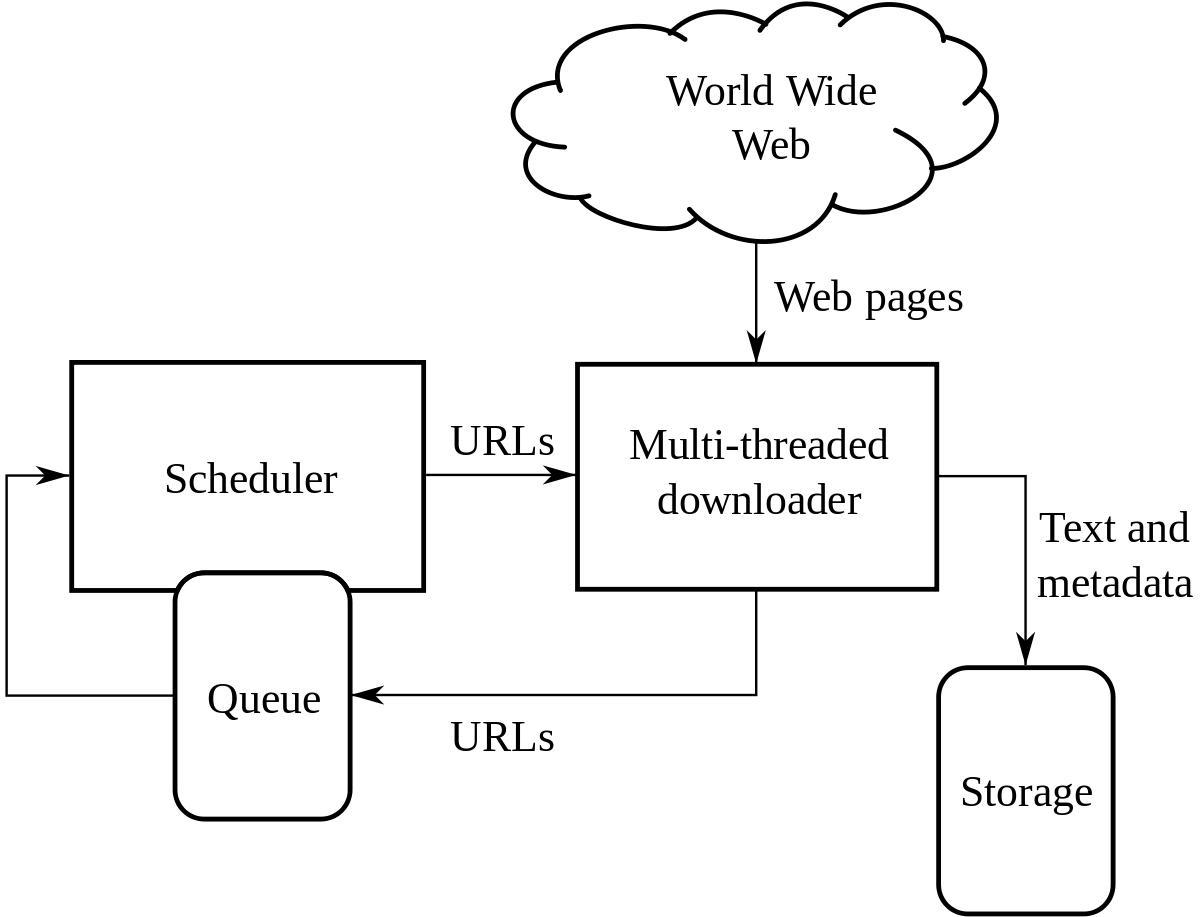
\includegraphics[width=0.5\columnwidth]{chapter2-analysis/WebCrawlerArchitecture.png} 
    \caption{Architettura di un web crawler.}
    \label{fig:architettura web crawler}
\end{figure}

%**************************************************************
\section{Cosa significa web scraping?}

Con il termine web scraping ci si riferisce all’estrapolazione di dati dai siti web. Il termine generalmente comprende anche l’estrapolazione fatta manualmente tramite software, anche se il termine principalmente si riferisce al processo automatizzato implementato tramite web crawler. Come esemplificato nella figura \ref{fig:funzionamento web scraper}, l’attività principale di cui si occupa un web scraper è la trasformazione di informazioni libere in informazioni strutturate per renderle di più facile utilizzo per una successiva analisi. I web scraper moderni devono occuparsi di estrapolare dati sia da fonti statiche che dinamiche, da questa necessità sono nate diverse tecniche per poter manipolare con successo dati provenienti da fonti non omogenee. La tecnica da me adottata è la combinazione delle tecniche chiamate ``Text pattern matching'' e ``HTTP programming''. Questa tecnica quindi riceve tramite richieste HTTP le pagine web e tramite \emph{regular expressions} ricerca determinati \emph{pattern}.

\begin{figure}[!h] 
    \centering 
    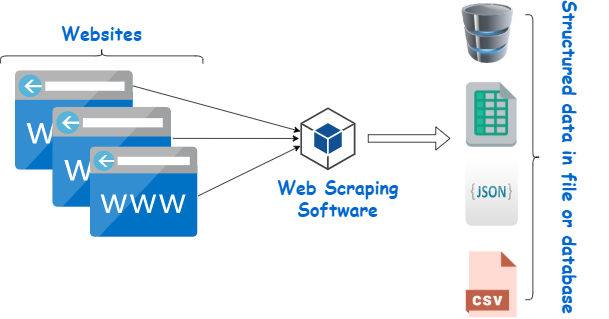
\includegraphics[width=0.6\columnwidth]{chapter2-analysis/webscraping.png} 
    \caption{Funzionamento di un web scraper.}
    \label{fig:funzionamento web scraper}
\end{figure}

%**************************************************************
\section{Deep web e dark web}
Il deep web è l'insieme delle risorse informative del World Wide Web (WWW) non indicizzate dai normali motori di ricerca. Il dark web invece è una porzione del deep web accessibile solamente tramite specifici software, configurazioni o autorizzazioni. Il dark web costituisce tra l`89 e il 96 percento del web ed è composto da diverse reti, sia piccole reti peer-to-peer e sia grandi reti come \gls{Tor}. Le due reti utilizzate durante il progetto sono \gls{Tor} e \gls{I2P}. \newline{}
Come per Internet ai suoi albori, il dark web ha una reputazione per essere un rifugio in cui svolgere attività illegali. Il dark web è stato coinvolto in diversi crimini ma anche utilizzato per evitare persecuzioni legate alla politica o alla propria identità. La crescita esponenziale delle gang del ransomware e di altri cyber criminali, rende sempre più necessario monitorare questa parte dell'internet. \newline{} Il monitoraggio risulta una necessità perchè questi criminali utilizzano il dark web per organizzarsi, pubblicare i nominativi delle vittime, comunicare con esse ed infine possibilmente pubblicarne i dati rubati. Lo scopo principale del sistema di monitoraggio è dunque quello di rilevare le tendenze in atto e l’esistenza di minacce impattanti un’organizzazione, prima che queste possano diventare fonte di danno per la stessa. Nel panorama attuale la Cyber Threat Intelligence costituisce un tassello fondamentale della Cyber Security e, grazie ad un approccio proattivo, diventa elemento differenziante nel contrasto alle minacce informatiche presenti nel dark web. \newline{}
L'accesso nel dark web, nel progetto di stage, è avvenuto configurando correttamente i proxy e avendo attivi i servizi di \gls{Tor} e di \gls{I2P}. Per selenium, utilizzando come webdriver chrome, è mostrato un esempio di configurazione nel listato \ref{listing: configurazione proxy selenium}; per requests, invece, viene mostrato un esempio di configurazione nel listato \ref{listing: configurazione proxy requests}.

\begin{lstlisting}[caption=Configurazione del proxy di selenium con webdriver chrome per l'accesso al dark web.,
	label=listing: configurazione proxy selenium]
if self.__is_tor_active:
    proxy = 'socks5://127.0.0.1:9050'
    options.add_argument('--proxy-server=%s' % proxy)
if self.__is_i2p_connection:
    proxy = 'http://127.0.0.1:4444'
    options.add_argument('--proxy-server=%s' % proxy)
\end{lstlisting}

\begin{lstlisting}[caption=Configurazione dei proxy di requests per l'accesso al dark web.,
	label=listing: configurazione proxy requests]
if self.__is_tor_active:
    self.session.proxies['http'] = 'socks5h://localhost:9050'
    self.session.proxies['https'] = 'socks5h://localhost:9050'
if self.__is_i2p_connection:
    self.session.proxies['http'] = 'http://localhost:4444'
    self.session.proxies['https'] = 'http://localhost:4444'
\end{lstlisting}
%**************************************************************
\section{Studio dei moduli preesistenti}

Prima di progettare e sviluppare il nuovo modulo di web crawling, è stato necessario effettuare un’analisi della piattaforma già presente all’interno dell’azienda, per comprenderne la struttura e le funzionalità offerte. Principalmente, è stato fondamentale individuare l’organizzazione delle funzionalità di \emph{log}, dei file di configurazione e del codice. La struttura del modulo preesistente è risultata pulita, di facile comprensione e molto scalabile, richiedendo per l’inserimento del nuovo modulo l’aggiunta di poche e coincise linee di codice. Nel listato \ref{listing: Aggiunta argomento webscraper} viene dimostrato come è stato aggiunto l'argomento a linea di comando per utilizzare il modulo, mentre nel listato \ref{listing: Aggiunta chiamata webscraper} è mostrata la logica secondo la quale viene richiamato il modulo avendo come input il testo inserito da linea di comando. Un comando da terminale, con questa sintassi, andrà quindi a richiamare correttamente il modulo di webscraping:
\centerline{\texttt{nome\_eseguibile -{}-webscraper -{}-altro\_modulo}}


\begin{lstlisting}[caption=Aggiunta dell’argomento da terminale.,
	label=listing: Aggiunta argomento webscraper]
group.add_argument('--webscraper', action='store_true',
                   help='catch info from the web')
\end{lstlisting}

\begin{lstlisting}[caption=Logica per l’utilizzo del webscraper.,
  	label=listing: Aggiunta chiamata webscraper]
elif arguments.webscraper:
    from modules import ywebscraper
    source_scrape = ywebscraper.YWebscraper(conf)
    source_scrape.process()
\end{lstlisting}

\section{Individuazione degli obiettivi}
Insieme al tutor aziendale sono stati elencati diversi requisiti atti a definire il lavoro da realizzare. Nella sezione \ref{subsec: Notazione obiettivi} vengono definiti i criteri con i quali sono stati catalogati mentre nella sezione \ref{subsec: Tabella obiettivi} vengono descritti ed identificati univocamente.
\subsection{Notazione obiettivi} \label{subsec: Notazione obiettivi}
Si farà riferimento ai requisiti secondo le notazioni in Tabella \ref{tab:notazione-requisiti}.
\begin{longtable}{|p{0.2\textwidth}|p{0.8\textwidth}|}
	\caption{Notazione dei requisiti}
	\label{tab:notazione-requisiti} \\
	\hline
    \textbf{Notazione}	&	\textbf{Descrizione} \\
    OB			&	Requisiti obbligatori, vincolanti in quanto obiettivo primario richiesto dal committente. \\  
	\hline
    D			&	Requisiti desiderabili, non vincolanti o strettamente necessari, ma dal riconoscibile valore aggiunto. \\ 
	\hline
    OP			&	Requisiti opzionali, rappresentanti valore aggiunto non strettamente competitivo. \\
    \hline
\end{longtable}%

\subsection{Tabella degli obiettivi} \label{subsec: Tabella obiettivi}
I requisiti, in ordine di priorità, vengono catalogati nella Tabella \ref{tab:tabella-obiettivi}.
\begin{longtable}{|p{0.2\textwidth}|p{0.8\textwidth}|}
	\caption{Tabella degli obiettivi}
	\label{tab:tabella-obiettivi} \\
	\hline
	\textbf{Codice}	&	\textbf{Descrizione} \\
    \hline
    OB01		&	Configurazione dell’ambiente di sviluppo \\  
	\hline
    OB02		&	Scrittura del documento ``Analisi dei Requisiti'' \\ 
	\hline
    OB03		&	Scrittura della guida ``README.md'' \\
    \hline
    OB04		&	Progettazione del modulo di web crawling intelligente \\
    \hline
    OB05		&	Funzionamento del modulo su rete Tor \\
    \hline
    OB06		&	Funzionamento utilizzando la libreria ``requests''  \\
    \hline
    OB07		&	Implementazione di Celery \\
    \hline
    OB08		&	Configurazione dei file di log \\
    \hline
    OB09		&	Ricerca url da analizzare tramite tag href \\
    \hline
    OB10		&	Implementazione della ricerca di informazioni interessanti tramite regex \\
    \hline
    OB11		&	Implementazione di priorità di analisi calcolate dinamicamente ed intelligentemente \\
    \hline
    OB12		&	Implementazione di un sistema per riprovare url con i quali è fallita la connessione \\
    \hline
    D01			&	Funzionamento del modulo su clear web \\
    \hline
    D02			&	Implementazione di un sistema di caching tramite redis degli url visitati \\
    \hline
    D03			&	Ricerca url da analizzare in tutto il codice sorgente della pagina \\
    \hline
    D04			&	Sanitizzazione degli url estrapolati \\
    \hline
    D05			&	Implementazione di una lista di siti di cui evitare l’analisi \\
    \hline 
    D06			&	Implementazione dell’utilizzo di Selenium \\
    \hline
    D07			&	Creazione di file di log in formato csv \\
    \hline
    D08			&	Implementazione di chiamate di rete intelligenti tramite gli headers HTTP \\
    \hline
    D09			&	Salvataggio ed utilizzo dei cookie di sessione \\
    \hline
    D10			&	Creazione dell’ambiente di test \\
    \hline
    OP01		&	Implementazione di molteplici browser tramite selenium \\
    \hline
    OP02		&	Funzionamento del modulo su rete I2P \\
    \hline
    OP03		&	Estensiva gestione delle eccezioni \\
    \hline
    OP04		&	Implementazione del salvataggio di file su directory temporanee \\
    \hline
    OP05		&	Salvataggio di screenshot e codice sorgente degli url interessanti su Amazon S3 \\
    \hline
    OP06		&	Scrittura dei test di unità \\
    \hline
\end{longtable}%

%**************************************************************
\section{Caratteristiche del modulo}
%**************************************************************

Il modulo, oltre a fornire tutte le funzionalità descritte precedentemente, deve avere le
seguenti caratteristiche: deve essere scalabile e performante, per permettere un aumento o diminuzione delle risorse; questo viene realizzato tramite una corretta progettazione, mirata alla ottimizzazione dell’utilizzo di memoria, per poter permettere a più istanze del programma di essere eseguite contemporaneamente tramite la libreria~\emph{Celery}.